\let\negmedspace\undefined
\let\negthickspace\undefined
\documentclass[journal]{IEEEtran}
\usepackage[a5paper, margin=10mm, onecolumn]{geometry}
%\usepackage{lmodern} % Ensure lmodern is loaded for pdflatex
\usepackage{tfrupee} % Include tfrupee package

\setlength{\headheight}{1cm} % Set the height of the header box
\setlength{\headsep}{0mm}     % Set the distance between the header box and the top of the text

\usepackage{gvv-book}
\usepackage{gvv}
\usepackage{cite}
\usepackage{amsmath,amssymb,amsfonts,amsthm}
\usepackage{algorithmic}
\usepackage{graphicx}
\usepackage{textcomp}
\usepackage{xcolor}
\usepackage{txfonts}
\usepackage{listings}
\usepackage{enumitem}
\usepackage{mathtools}
\usepackage{gensymb}
\usepackage{comment}
\usepackage[breaklinks=true]{hyperref}
\usepackage{tkz-euclide} 
\usepackage{listings}
% \usepackage{gvv}                                        
\def\inputGnumericTable{}                                 
\usepackage[latin1]{inputenc}                                
\usepackage{color}                                            
\usepackage{array}                                            
\usepackage{longtable}                                       
\usepackage{calc}                                             
\usepackage{multirow}                                         
\usepackage{hhline}                                           
\usepackage{ifthen}                                           
\usepackage{lscape}
\begin{document}

\bibliographystyle{IEEEtran}
\vspace{3cm}

\title{1-1.9-11}
\author{EE24BTECH11060 - Sruthi Bijili}
% \maketitle
% \newpage
% \bigskip
{\let\newpage\relax\maketitle}

\renewcommand{\thefigure}{\theenumi}
\renewcommand{\thetable}{\theenumi}
\setlength{\intextsep}{10pt} % Space between text and floats


\numberwithin{equation}{enumi}
\numberwithin{figure}{enumi}
\renewcommand{\thetable}{\theenumi}

\textbf{Question}:\\
If the distance between the points \brak{k,-2} and \brak{3,-6} is $10$ units, find the positive value of $k$.
\hfill(10,2021)\\
\textbf{solution:}
\begin{table}[h!]    
  \centering
  \begin{tabular}[12pt]{ |c| c|}
    \hline
        \textbf{Variable}  & \textbf{Description} \\
    \hline
        $\vec{A}$$\brak{-5,4}$ &  coordinates of first point \\
    \hline 
        $\vec{B}$$\brak{-1,6}$ & coordinates of second point \\
    \hline
        $\vec{C}$& midpoint of $\vec{A}$ and $\vec{B}$ \\ 
    \hline       
\end{tabular}

  \caption{Input parameters}
\end{table}
\begin{align}
\abs{\abs{AB}}&=\sqrt{\brak{A-B}^T\brak{A-B}}\\
\implies \abs{\abs{AB}}&=\sqrt{\brak{A^T-B^T}\brak{A-B}}\\
\implies \abs{\abs{AB}}&=\sqrt{A^TA-A^TB-B^TA+B^TB}\\
\implies \abs{\abs{AB}}&=\sqrt{A^TA-2A^TB+B^TB}\\
\implies 10 &=\sqrt{\myvec{k \\ -2}^T\myvec{3 \\-6}-2\myvec{K \\-2}^T\myvec{3\\-6}+\myvec{3\\-6}^T\myvec{3\\-6}}\\
\implies 10 &=\sqrt{k^2-6k+25}\\
k^2-6k-75&=0\\
\implies k&=3-2\sqrt{21},3+2\sqrt{21}
\end{align}
\text{Therefore the positive value of $k$ is $3+2\sqrt{21}$}
\begin{figure}[h!]
   \centering
   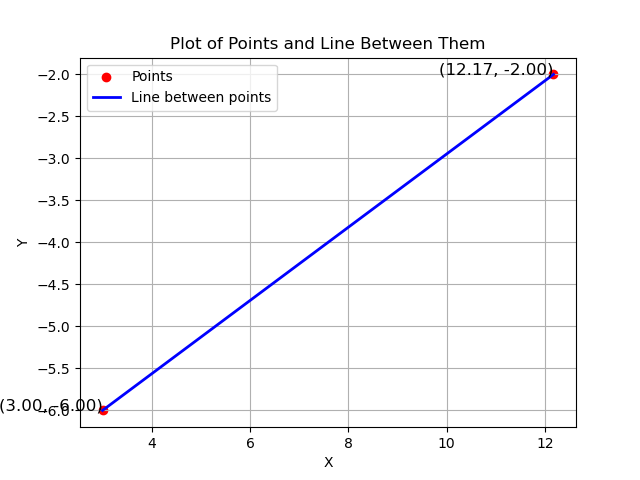
\includegraphics[width=0.7\linewidth]{figs/fig1.png}
   \caption{line AB}
\end{figure}

\end{document}

